\section{演员-评论员算法}
在REINFORCE算法中,每次需要根据一个策略采集一条完整的轨迹,并计算这条轨迹上的回报。这种采样方式的方差比较大,学习效率也比较低。我们可以借鉴时序差分学习的思想,使用动态规划方法来提高采样效率,即从状态 $s$ 开始的总回报可以通过当前动作的即时奖励 $r(s,a,s')$ 和下一个状态 $s'$ 的值函数来近似估计。

\kw{演员-评论员算法}是一种结合\kw{策略梯度}和\kw{时序差分学习}的强化学习方法,其中,
演员是指策略函数 $\pi_{\theta}(a|s)$,即学习一个策略以得到尽可能高的回报。
评论员是指价值函数 $V_{\pi}(s)$,对当前策略的值函数进行估计,即评估演员的好坏。
借助于价值函数,演员-评论员算法可以进行单步参数更新,不需要等到回合结束才进行更新。
在演员-评论员算法里面,最知名的算法就是异步优势演员-评论员算法。
如果我们去掉异步,则为\kw{优势演员-评论员(advantage actor-critic,A2C)算法}。A2C算法又被译作优势演员-评论员算法。
如果我们加了异步,变成异步优势演员-评论员算法。

\subsection{策略梯度回顾} 
我们复习一下策略梯度,在更新策略参数 $\theta$ 的时候,我们可以通过
\begin{equation}
  \label{eq:policy_gradient}
  \nabla \bar{R}_{\theta} \approx \frac{1}{N} \sum_{n=1}^{N} \sum_{t=1}^{T_{n}}\left(\sum_{t^{\prime}=t}^{T_{n}} \gamma^{t^{\prime}-t} r_{t^{\prime}}^{n}-b\right) \nabla \log p_{\theta}\left(a_{t}^{n} \mid s_{t}^{n}\right)
\end{equation}
来计算梯度。
\eqref{eq:policy_gradient} 表示我们首先通过智能体与环境的交互,可以计算出在某一个状态 $s$ 采取某一个动作 $a$ 的概率  $p_{\theta}(a_t|s_t)$。接下来,我们计算在某一个状态 $s$ 采取某一个动作 $a$ 之后直到游戏结束的累积奖励。$\sum_{t^{\prime}=t}^{T_{n}} \gamma^{t^{\prime}-t} r_{t^{\prime}}^{n}$ 表示我们把从时间 $t$ 到时间 $T$ 的奖励相加,并且在前面乘一个折扣因子,通常将折扣因子设置为 0.9 或 0.99等数值,与此同时也会减去一个基线值 $b$,减去值 $b$ 的目的是希望括号里面这一项是有正有负的。如果括号里面这一项是正的,我们就要增大在这个状态采取这个动作的概率;如果括号里面是负的,我们就要减小在这个状态采取这个动作的概率。

我们使用 $G$ 表示累积奖励,$G$ 是非常不稳定的。因为交互的过程本身具有随机性,所以在某一个状态 $s$ 采取某一个动作 $a$ 时计算得到的累积奖励,每次结果都是不同的,因此 $G$ 是一个随机变量。对于同样的状态 $s$ 和同样的动作 $a$,$G$ 可能有一个固定的分布。但由于我们采取采样的方式,因此我们在某一个状态 $s$ 采取某一个动作 $a$ 一直到游戏结束,统计一共得到了多少的奖励,我们就把它当作 $G$。

如\figref{fig:fig9.1} 所示,如果我们把 $G$ 想成一个随机变量,实际上是在对 $G$ 做采样,用这些采样的结果去更新参数。但实际上在某一个状态 $s$ 采取某一个动作 $a$,接下来会发生什么事,其本身是有随机性的。虽然说有一个固定的分布,但其方差可能会非常大。智能体在同一个状态采取同一个动作时,最后得到的结果可能会是很不一样的。
当然,假设我们在每次更新参数之前,都可以采样足够多次,那当然就没有以上的问题了。但我们每次做策略梯度,每次更新参数之前都要做一些采样时,采样的次数是不可能太多的,我们只能够做非常少量的采样。如果我们正好采样到差的结果,比如采样到 $G = 100$、采样到 $G = -10$,显然结果会是很差的。

\begin{figure}[hbt]
  \centering
  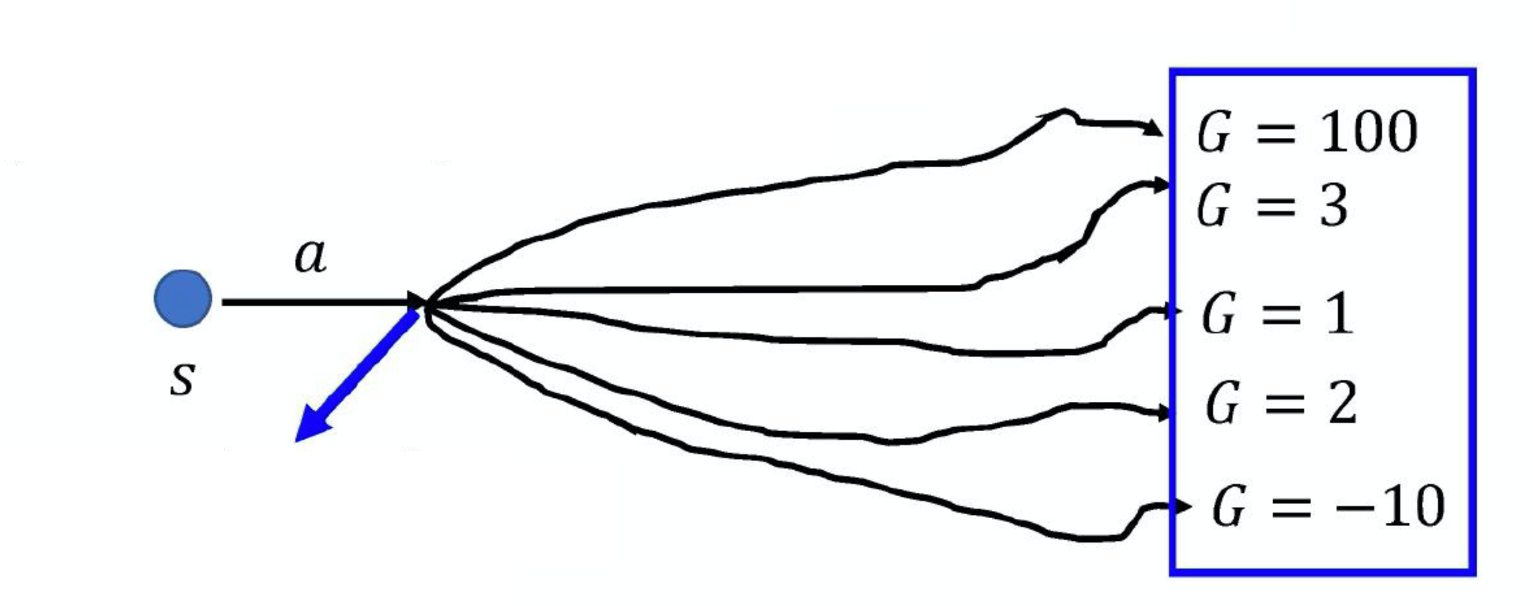
\includegraphics[width=0.4\linewidth]{res/ch9/9.1}
  \caption{策略梯度回顾}
  \label{fig:fig9.1}
\end{figure}

\subsection{深度Q网络回顾}

Q:我们能不能让整个训练过程变得稳定,能不能直接估测随机变量 $G$ 的期望值?

A:我们直接用一个网络去估测在状态 $s$ 采取动作 $a$ 时 $G$ 的期望值。如果这样是可行的,那么在随后的训练中我们就用期望值代替采样的值,这样就会让训练变得更加稳定。

Q:怎么使用期望值代替采样的值呢?

A:这里就需要引入基于价值的(value-based)的方法。基于价值的方法就是 深度Q网络 。深度Q网络 有两种函数,有两种评论员。
如\figref{fig:fig9.2} 所示,
  第一种评论员是 $V_{\pi}(s)$。即假设演员的策略是 $\pi$,使用 $\pi$ 与环境交互,当智能体看到状态 $s$ 时,接下来累积奖励的期望值是多少。
  第二种评论员是 $Q_{\pi}(s,a)$。$Q_{\pi}(s,a)$ 把 $s$ 与 $a$ 当作输入,它表示在状态 $s$ 采取动作 $a$,接下来用策略 $\pi$ 与环境交互,累积奖励的期望值是多少。
  $V_{\pi}$ 接收输入 $s$,输出一个标量。
  $Q_{\pi}$ 接收输入 $s$,它会给每一个 $a$ 都分配一个 Q值。
%   我们可以用时序差分或蒙特卡洛来估计。两者的区别是,用时序差分比较稳定,用 蒙特卡洛 比较精确。


\begin{figure}[hbt]
  \centering
  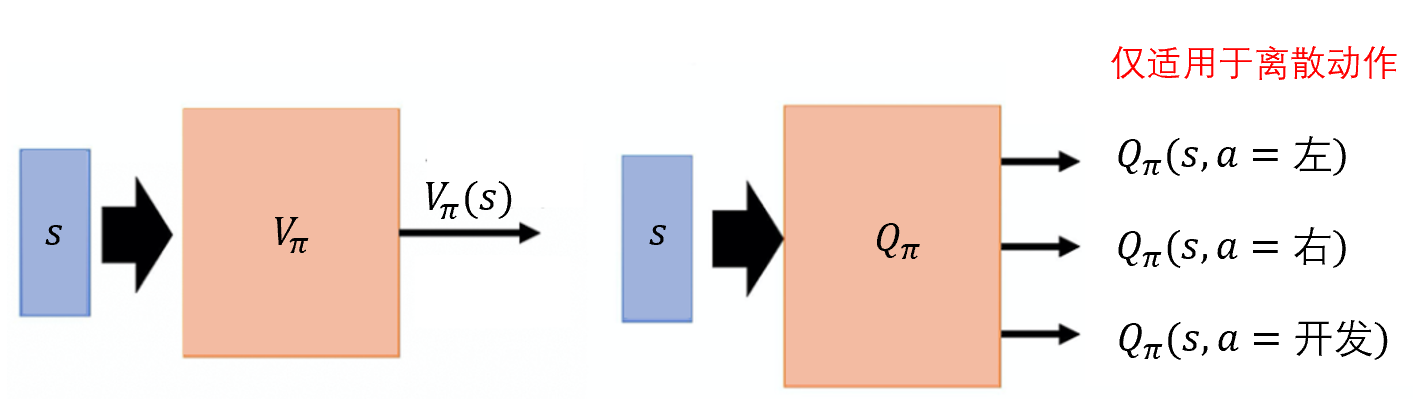
\includegraphics[width=0.7\linewidth]{res/ch9/9.2}
  \caption{深度Q网络}
  \label{fig:fig9.2}
\end{figure}

\subsection{优势演员-评论员算法}
如\figref{fig:fig9.3} 所示,
随机变量 $G$ 的期望值正好就是 Q 值,即
\begin{equation}
  \label{eq:}
  \mathbb{E}\left[G_{t}^{n}\right]=Q_{\pi_{\theta}} \left(s_{t}^{n}, a_{t}^{n}\right)
\end{equation}
此也为 Q 函数的定义。Q函数的定义就是在某一个状态 $s$,采取某一个动作 $a$,假设策略是 $\pi$ 的情况下所能得到的累积奖励的期望值,即 $G$ 的期望值。累积奖励的期望值就是 $G$ 的期望值。
所以假设用 $\mathbb{E}\left[G_{t}^{n}\right]$ 来代表 $\sum_{t^{\prime}=t}^{T_{n}} \gamma^{t^{\prime}-t} r_{t^{\prime}}^{n}$ 这一项,把Q函数套在这里就结束了,我们就可以把演员与评论员这两个方法结合起来。

有不同的方法表示基线,一个常见的方法是用价值函数 $V_{\pi_{\theta}}\left(s_{t}^{n}\right)$ 来表示基线。价值函数的定义为,假设策略是 $\pi$,其在某个状态 $s$ 一直与环境交互直到游戏结束,期望奖励有多大。 $V_{\pi_{\theta}}\left(s_{t}^{n}\right)$ 没有涉及动作,$Q_{\pi_{\theta}}\left(s_{t}^{n}, a_{t}^{n}\right)$ 涉及动作。
$V_{\pi_{\theta}}\left(s_{t}^{n}\right)$ 是 $Q_{\pi_{\theta}}\left(s_{t}^{n}, a_{t}^{n}\right)$ 的期望值, $Q_{\pi_{\theta}}\left(s_{t}^{n}, a_{t}^{n}\right)-V_{\pi_{\theta}}\left(s_{t}^{n}\right)$ 会有正有负,所以 $\sum_{t^{\prime}=t}^{T_{n}} \gamma^{t^{\prime}-t} r_{t^{\prime}}^{n}-b$ 这一项就会有正有负。
所以我们就把策略梯度里面 $\sum_{t^{\prime}=t}^{T_{n}} \gamma^{t^{\prime}-t} r_{t^{\prime}}^{n}-b$ 这一项换成了优势函数$A^{\theta}\left(s^{n}_{t}, a^{n}_{t}\right)$,即 $Q_{\pi_{\theta}}\left(s_{t}^{n}, a_{t}^{n}\right)-V_{\pi_{\theta}}\left(s_{t}^{n}\right)$。因此该算法称为优势演员-评论员算法。
\begin{figure}[hbt]
  \centering
  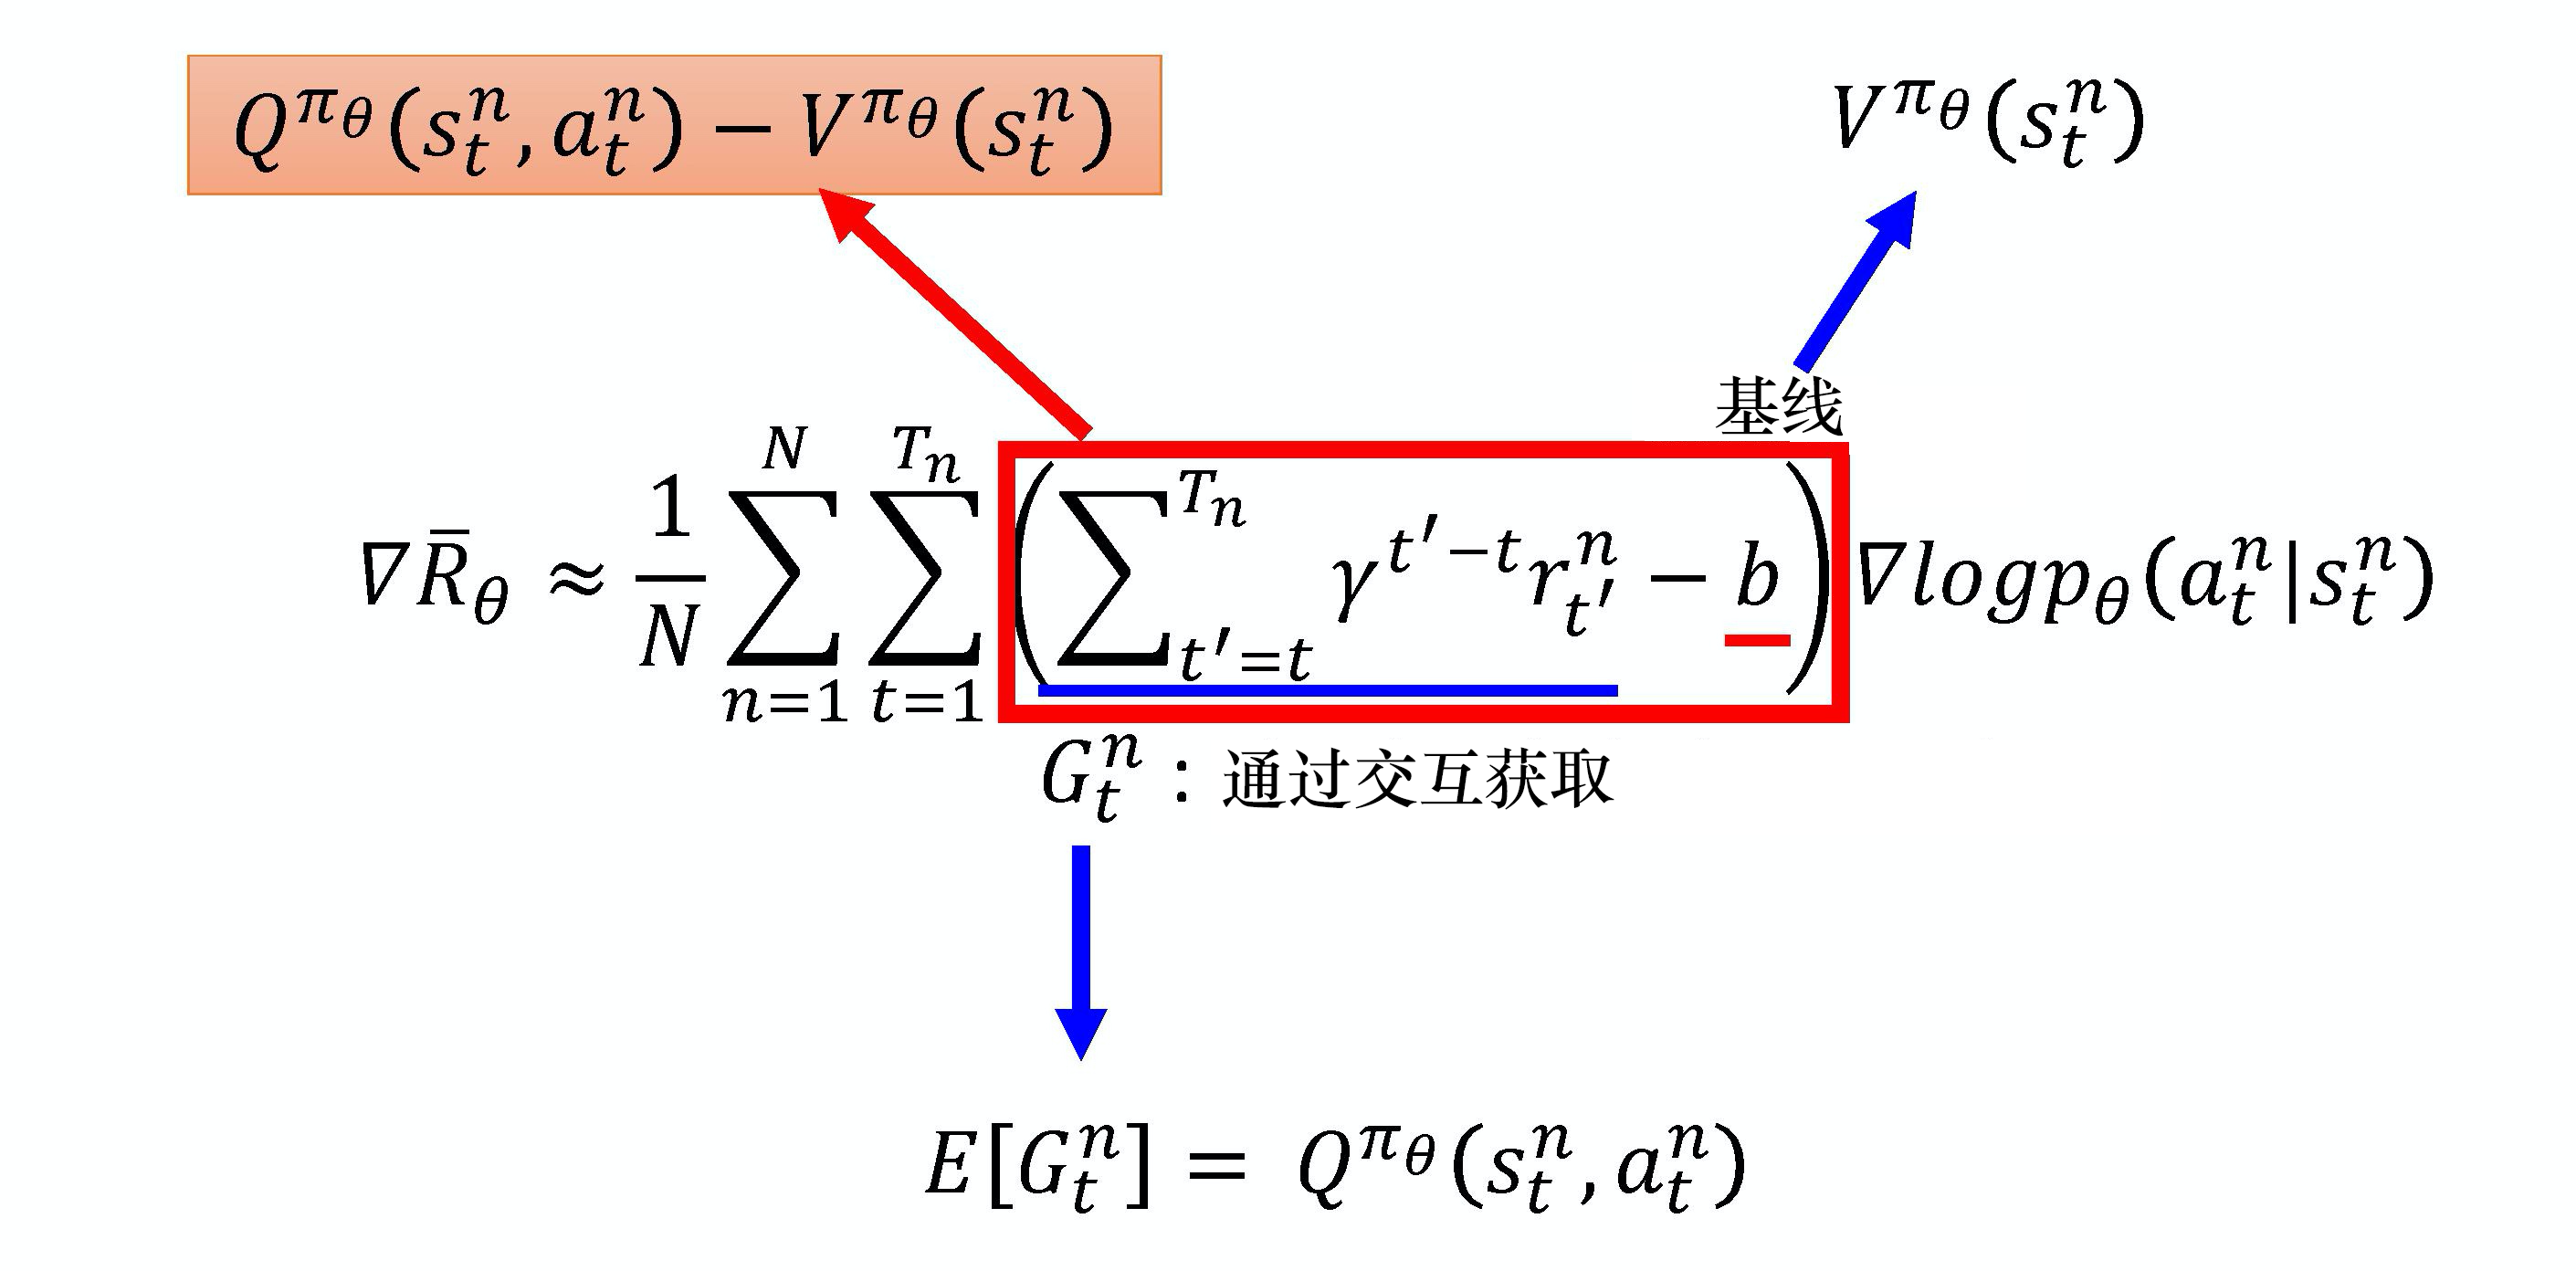
\includegraphics[width=0.5\linewidth]{res/ch9/9.3}
  \caption{优势演员-评论员算法}
  \label{fig:fig9.3}
\end{figure}

如果我们这么实现,有一个缺点,即我们需要估计两个网络------Q网络和 V网络,估计不准的风险就变成原来的两倍。所以我们何不只估计一个网络呢?
事实上,在演员-评论员算法中,我们可以只估计网络 V,并利用 $V$ 的值来表示 $Q$ 的值,$Q_{\pi}\left(s_{t}^{n}, a_{t}^{n}\right)$ 可以写成 $ r_{t}^{n}+V_{\pi}\left(s_{t+1}^{n}\right)$ 的期望值,即
\begin{equation}
  \label{eq:}
  Q_{\pi}\left(s_{t}^{n}, a_{t}^{n}\right)=\mathbb{E}\left[r_{t}^{n}+V_{\pi}\left(s_{t+1}^{n}\right)\right]
\end{equation}

在状态 $s$ 采取动作 $a$,我们会得到奖励 $r$,进入状态 $s_{t+1}$。但是我们会得到什么样的奖励 $r$,进入什么样的状态 $s_{t+1}$,这件事本身是有随机性的。所以要把$r_{t}^{n}+V_{\pi}\left(s_{t+1}^{n}\right)$取期望值才会等于Q函数的值。但我们现在把取期望值去掉,即
\begin{equation}
  \label{eq:}
  Q_{\pi}\left(s_{t}^{n}, a_{t}^{n}\right)=r_{t}^{n}+V_{\pi}\left(s_{t+1}^{n}\right)
\end{equation}

我们就可以把Q函数的值用 $r_t^n + V_{\pi}\left(s_{t+1}^{n}\right)$ 取代,可得
\begin{equation}
  \label{eq:}
  r_{t}^{n}+V_{\pi}\left(s_{t+1}^{n}\right)-V_{\pi}\left(s_{t}^{n}\right)
\end{equation}

把取期望值去掉的好处就是我们不需要估计 $Q$ 了,只需要估计 $V$。但与此同时我们会引入一个随机的参数 $r$。$r$ 是有随机性的,它是一个随机变量,但是 $r$ 相较于累积奖励 $G$ 是一个较小的值,因为它是某一个步骤得到的奖励,而 $G$ 是所有未来会得到的奖励的总和,$G$ 的方差比较大。$r$ 虽然也有一些方差,但它的方差比 $G$ 的要小。所以把原来方差比较大的 $G$ 换成方差比较小的 $r$ 也是合理的。

Q:为什么我们可以直接把取期望值去掉?

A:原始的异步优势演员-评论员算法的论文尝试了各种方法,最后发现这个方法最好。当然有人可能会有疑问,说不定估计 $Q$ 和 $V$ 也可以估计得很好,但实际做实验的时候,最后结果就是这个方法最好,所以后来大家都使用了这个方法。

优势演员-评论员算法的流程如\figref{fig:fig9.5} 所示,我们有一个 $\pi$,有个初始的演员与环境交互,先收集资料。在策略梯度方法里收集资料以后,就来更新策略。但是在演员-评论员算法里面,我们不是直接使用那些资料来更新策略。我们先用这些资料去估计价值函数,可以用 时序差分方法 或 蒙特卡洛方法 来估计价值函数。接下来,我们再基于价值函数,使用\eqref{eq:update_pi} 更新 $\pi$。
\begin{equation}
  \label{eq:update_pi}
  \nabla \bar{R}_{\theta} \approx \frac{1}{N} \sum_{n=1}^{N} \sum_{t=1}^{T_{n}}\left(r_{t}^{n}+V_{\pi}\left(s_{t+1}^{n}\right)-V_{\pi}\left(s_{t}^{n}\right)\right) \nabla \log p_{\theta}\left(a_{t}^{n} \mid s_{t}^{n}\right)
\end{equation}
有了新的 $\pi$ 以后,再与环境交互,收集新的资料,去估计价值函数。再用新的价值函数更新策略,更新演员。
整个优势演员-评论员算法就是这么运作的。

\begin{figure}[h]
  \centering
  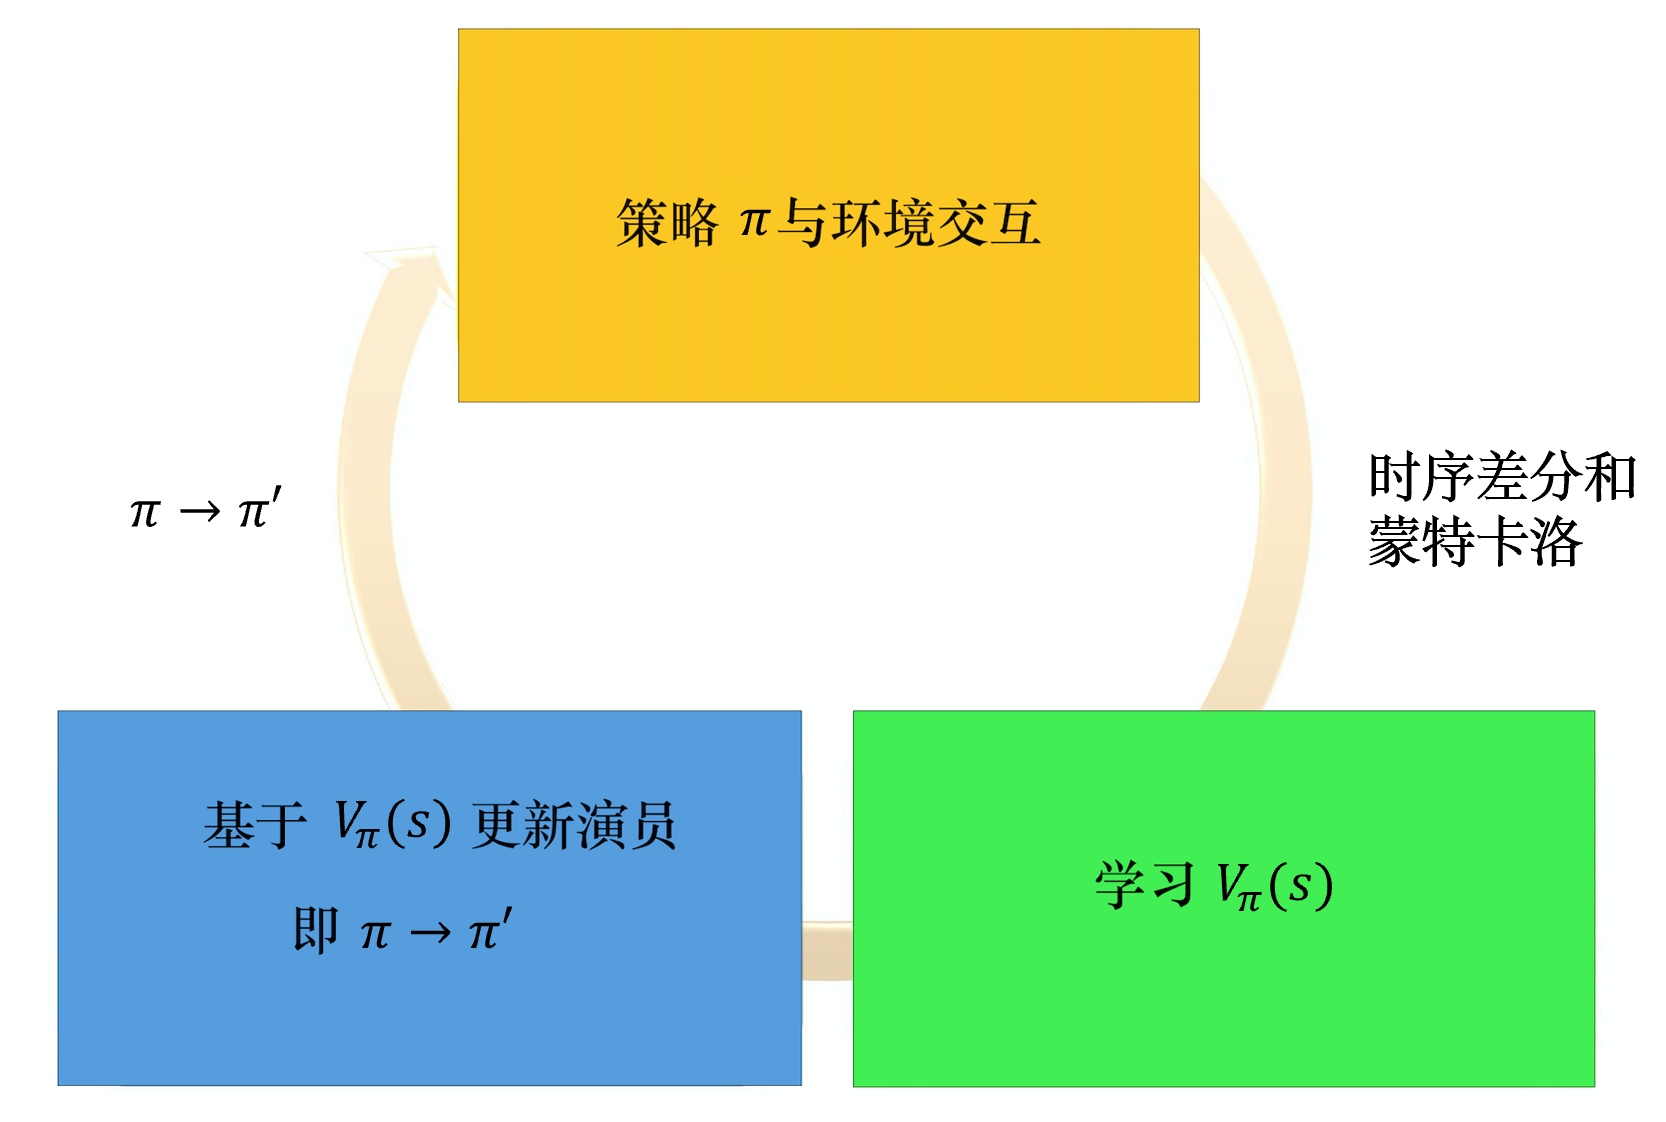
\includegraphics[width=0.4\linewidth]{res/ch9/9.5}
  \caption{优势评论员-评论员算法流程}
  \label{fig:fig9.5}
\end{figure}

实现优势演员-评论员算法的时候,有两个一定会用到的技巧。
第一个技巧是,我们需要估计两个网络:$V$ 网络和策略的网络(也就是演员)。
  评论员网络 $V_\pi(s)$ 接收一个状态,输出一个标量。
  演员的策略 $\pi(s)$ 接收一个状态,
  如果动作是离散的,输出就是一个动作的分布,
  如果动作是连续的,输出就是一个连续的向量。

\figref{fig:fig9.6} 所示为离散动作的例子,连续动作的情况也是一样的。输入一个状态,网络决定现在要采取哪一个动作。演员网络和评论员网络的输入都是 $s$,所以它们前面几个层(layer)是可以共享的。
\begin{figure}[h]
  \centering
  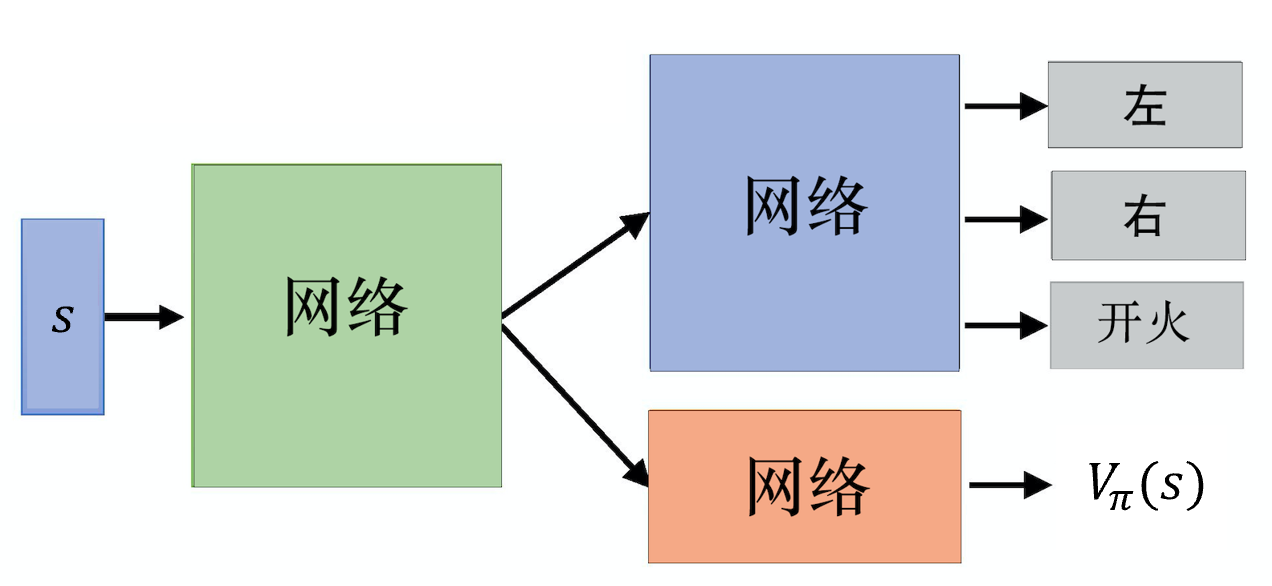
\includegraphics[width=0.5\linewidth]{res/ch9/9.6}
  \caption{离散动作的例子}
  \label{fig:fig9.6}
\end{figure}

尤其当我们在玩雅达利游戏时,输入都是图像。输入的图像非常复杂,通常我们在前期都会用一些卷积神经网络来处理它们,把图像抽象成高级(high level)的信息。把像素级别的信息抽象成高级信息的特征提取器,对于演员与评论员来说是可以共用的。所以通常我们会让演员与评论员共享前面几层,并且共用同一组参数,这一组参数大部分都是卷积神经网络的参数。
先把输入的像素变成比较高级的信息,再让演员决定要采取什么样的动作,让评论员即价值函数计算期望奖励。

第二个技巧是我们需要探索的机制。在演员-评论员算法中,有一个常见的探索的方法是对 $\pi$ 输出的分布设置一个约束。这个约束用于使分布的熵(entropy)不要太小,也就是希望不同的动作被采用的概率平均一些。这样在测试的时候,智能体才会多尝试各种不同的动作,才会把环境探索得比较好,从而得到比较好的结果。

\subsection{异步优势演员-评论员算法} 
强化学习有一个问题,就是它很慢,怎么提高训练的速度呢?例如,如\figref{fig:fig9.7} 所示,在动漫《火影忍者》中,有一次鸣人想要在一周之内打败晓,所以要加快修行的速度,鸣人的老师就教他一个方法:用影分身进行同样的修行。两个一起修行,经验值累积的速度就会变成两倍,所以鸣人就使用了 1000 个影分身来进行修行。这就是异步优势演员-评论员算法的体现。
\begin{figure}[hbt]
    \centering
    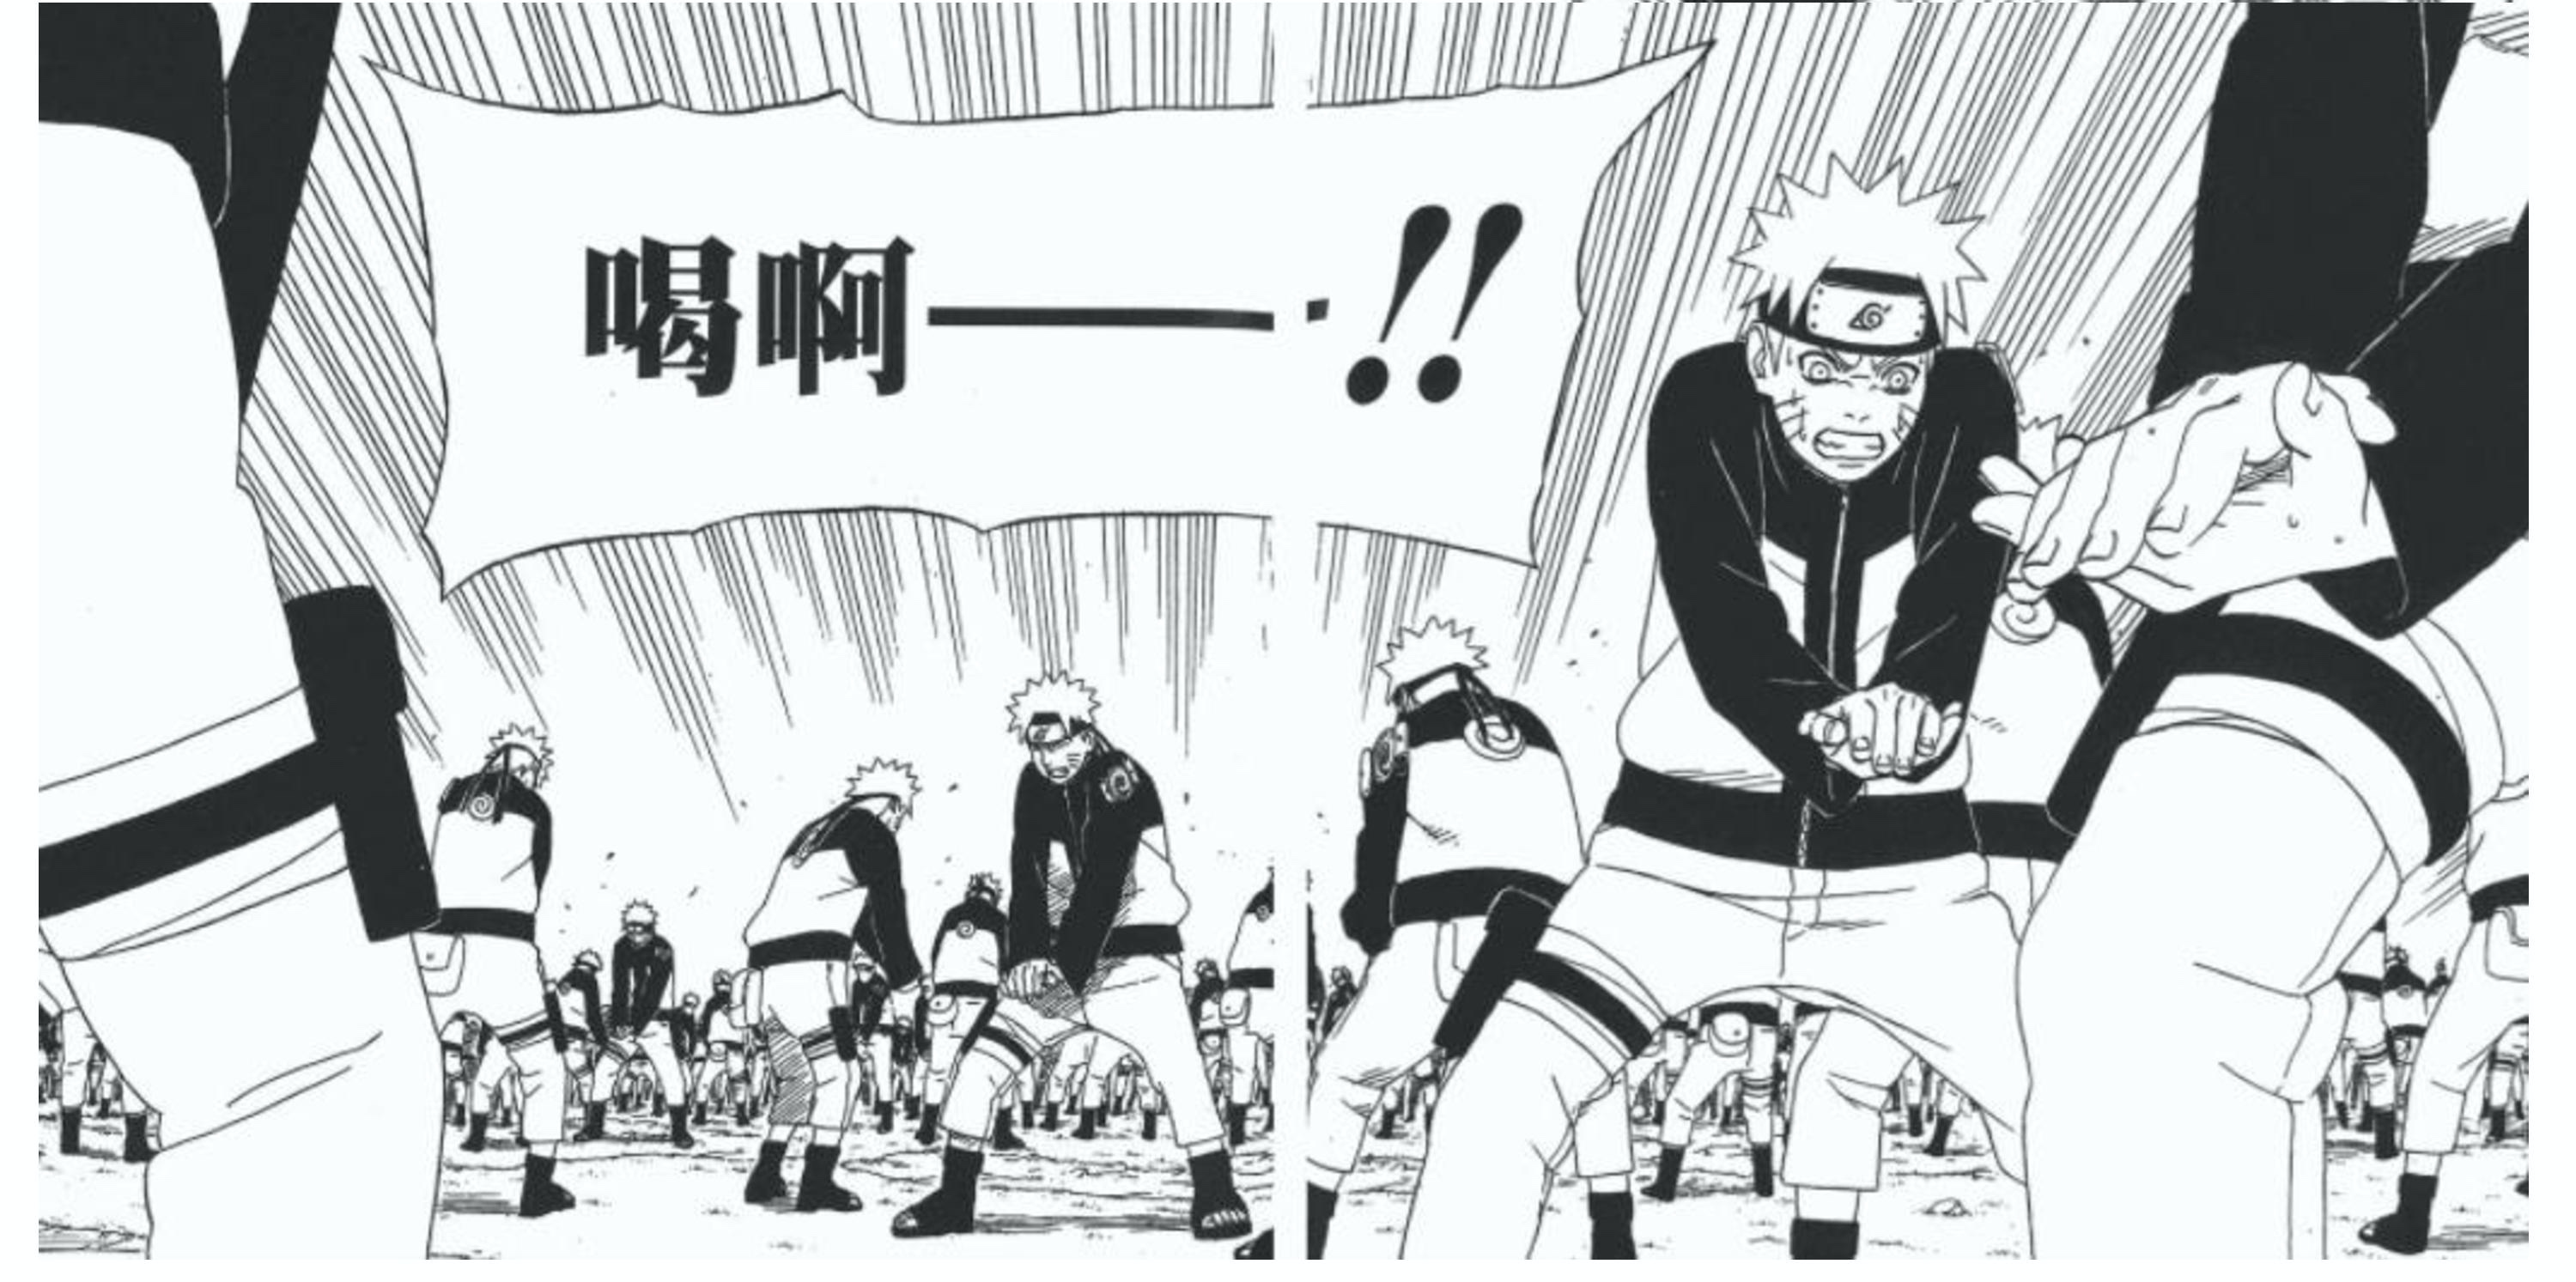
\includegraphics[width=0.5\linewidth]{res/ch9/9.7}
    \caption{影分身例子}
    \label{fig:fig9.7}
\end{figure}

异步优势演员-评论员算法同时使用很多个进程(worker),每一个进程就像一个影分身,最后这些影分身会把所有的经验值集合在一起。如果我们没有很多 CPU,不好实现异步优势演员-评论员算法,但可以实现优势演员-评论员算法。

异步优势演员-评论员算法的运作流程,如\figref{fig:fig9.8} 所示,
  异步优势演员-评论员算法一开始有一个全局网络(global network)。全局网络包含策略网络和价值网络,这两个网络是绑定(tie)在一起的,它们的前几个层会被绑在一起。
  假设全局网络的参数是 $\theta_1$,我们使用多个进程,每个进程用一张 CPU 去跑。比如我们有 8 个进程,则至少 8 张 CPU。每一个进程在工作前都会把全局网络的参数复制过来。
  接下来演员就与环境交互,每一个演员与环境交互的时候,都要收集到比较多样的数据。例如,如果是走迷宫,可能每一个演员起始的位置都会不一样,这样它们才能够收集到比较多样的数据。
  每一个演员与环境交互完之后,我们就会计算出梯度。计算出梯度以后,要用梯度去更新参数。我们就计算一下梯度,用梯度去更新全局网络的参数。就是这个进程算出梯度以后,就把梯度传回给中央的控制中心,中央的控制中心就会用这个梯度去更新原来的参数。
  
  注意,A3C使用了平行探索的方法,

  所有的演员都是平行跑的,每一个演员各做各的,不管彼此。所以每个演员都是去要了一个参数以后,做完就把参数传回去。当第一个进程做完想要把参数传回去的时候,本来它要的参数是 $\theta_1$,等它要把梯度传回去的时候,可能别人已经把原来的参数覆盖掉,变成 $\theta_2$了。但是没有关系,它一样会把这个梯度就覆盖过去。


\begin{figure}[hbt]
  \centering
  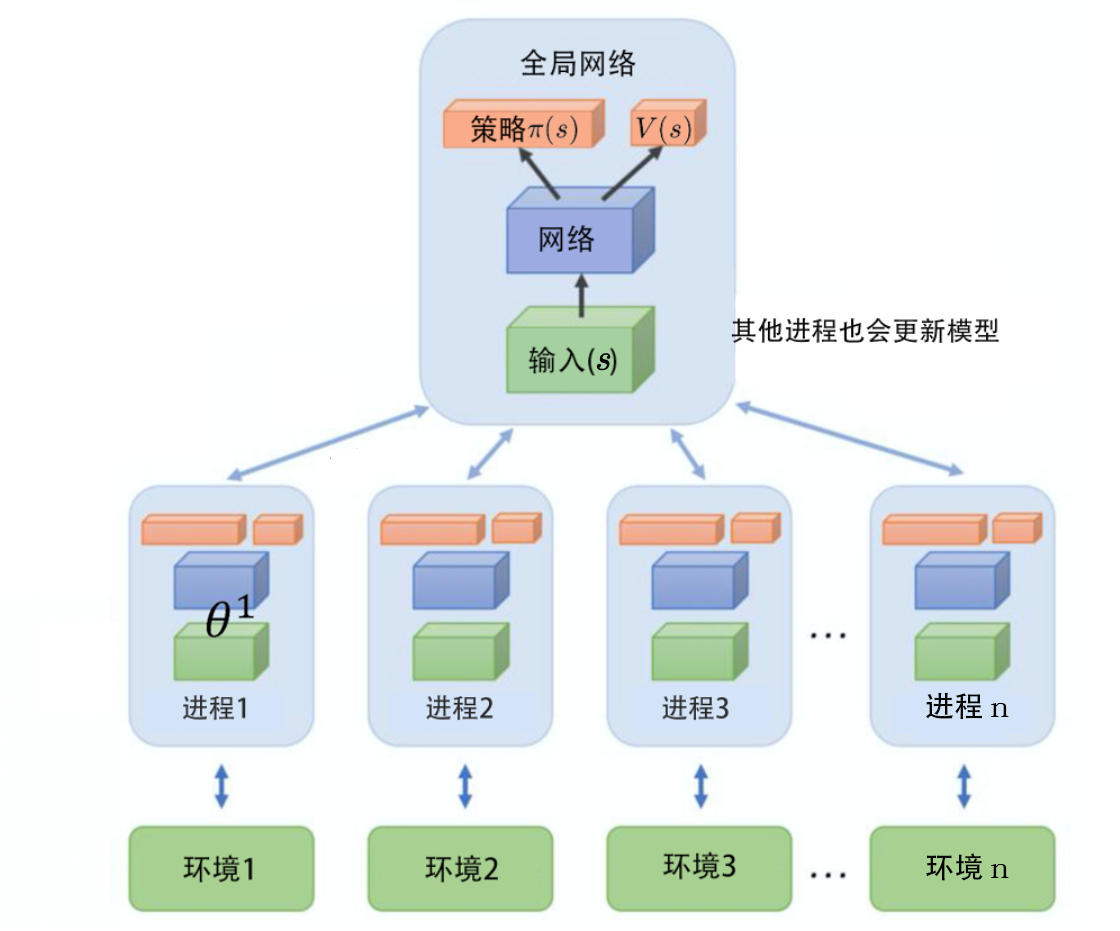
\includegraphics[width=0.4\linewidth]{res/ch9/9.8}
  \caption{异步优势演员-评论员算法的运作流程}
  \label{fig:fig9.8}
\end{figure}

\subsection{路径衍生策略梯度} 

接下来我们来了解\kw{路径衍生策略梯度(pathwise derivative policy gradient)}方法。这个方法可以看成 深度Q网络 解连续动作的一种特别的方法,也可以看成一种特别的演员-评论员的方法。
用动漫《棋魂》来比喻,阿光就是一个演员,佐为就是一个评论员。阿光落某一子以后,如果佐为是一般的演员-评论员算法的评论员,他会告诉阿光这时候不应该下小马步飞。佐为会告诉我们,我们现在采取的这一步算出来的值到底是好还是不好,但这样就结束了,他只告诉我们好还是不好。因为一般的演员-评论员算法的评论员就是输入状态或输入状态-动作对,给演员一个值,所以对演员来说,它只知道它做的这个动作到底是好还是不好。

但在路径衍生策略梯度里面,评论员会直接告诉演员采取什么样的动作才是好的。所以佐为不只是告诉阿光,这个时候不要下小马步飞,同时还告诉阿光这个时候应该要下大马步飞,这就是路径衍生策略梯度中的评论员所做的。评论员会直接告诉演员做什么样的动作才可以得到比较大的值。

% \begin{figure}[hbt]
%   \centering
%   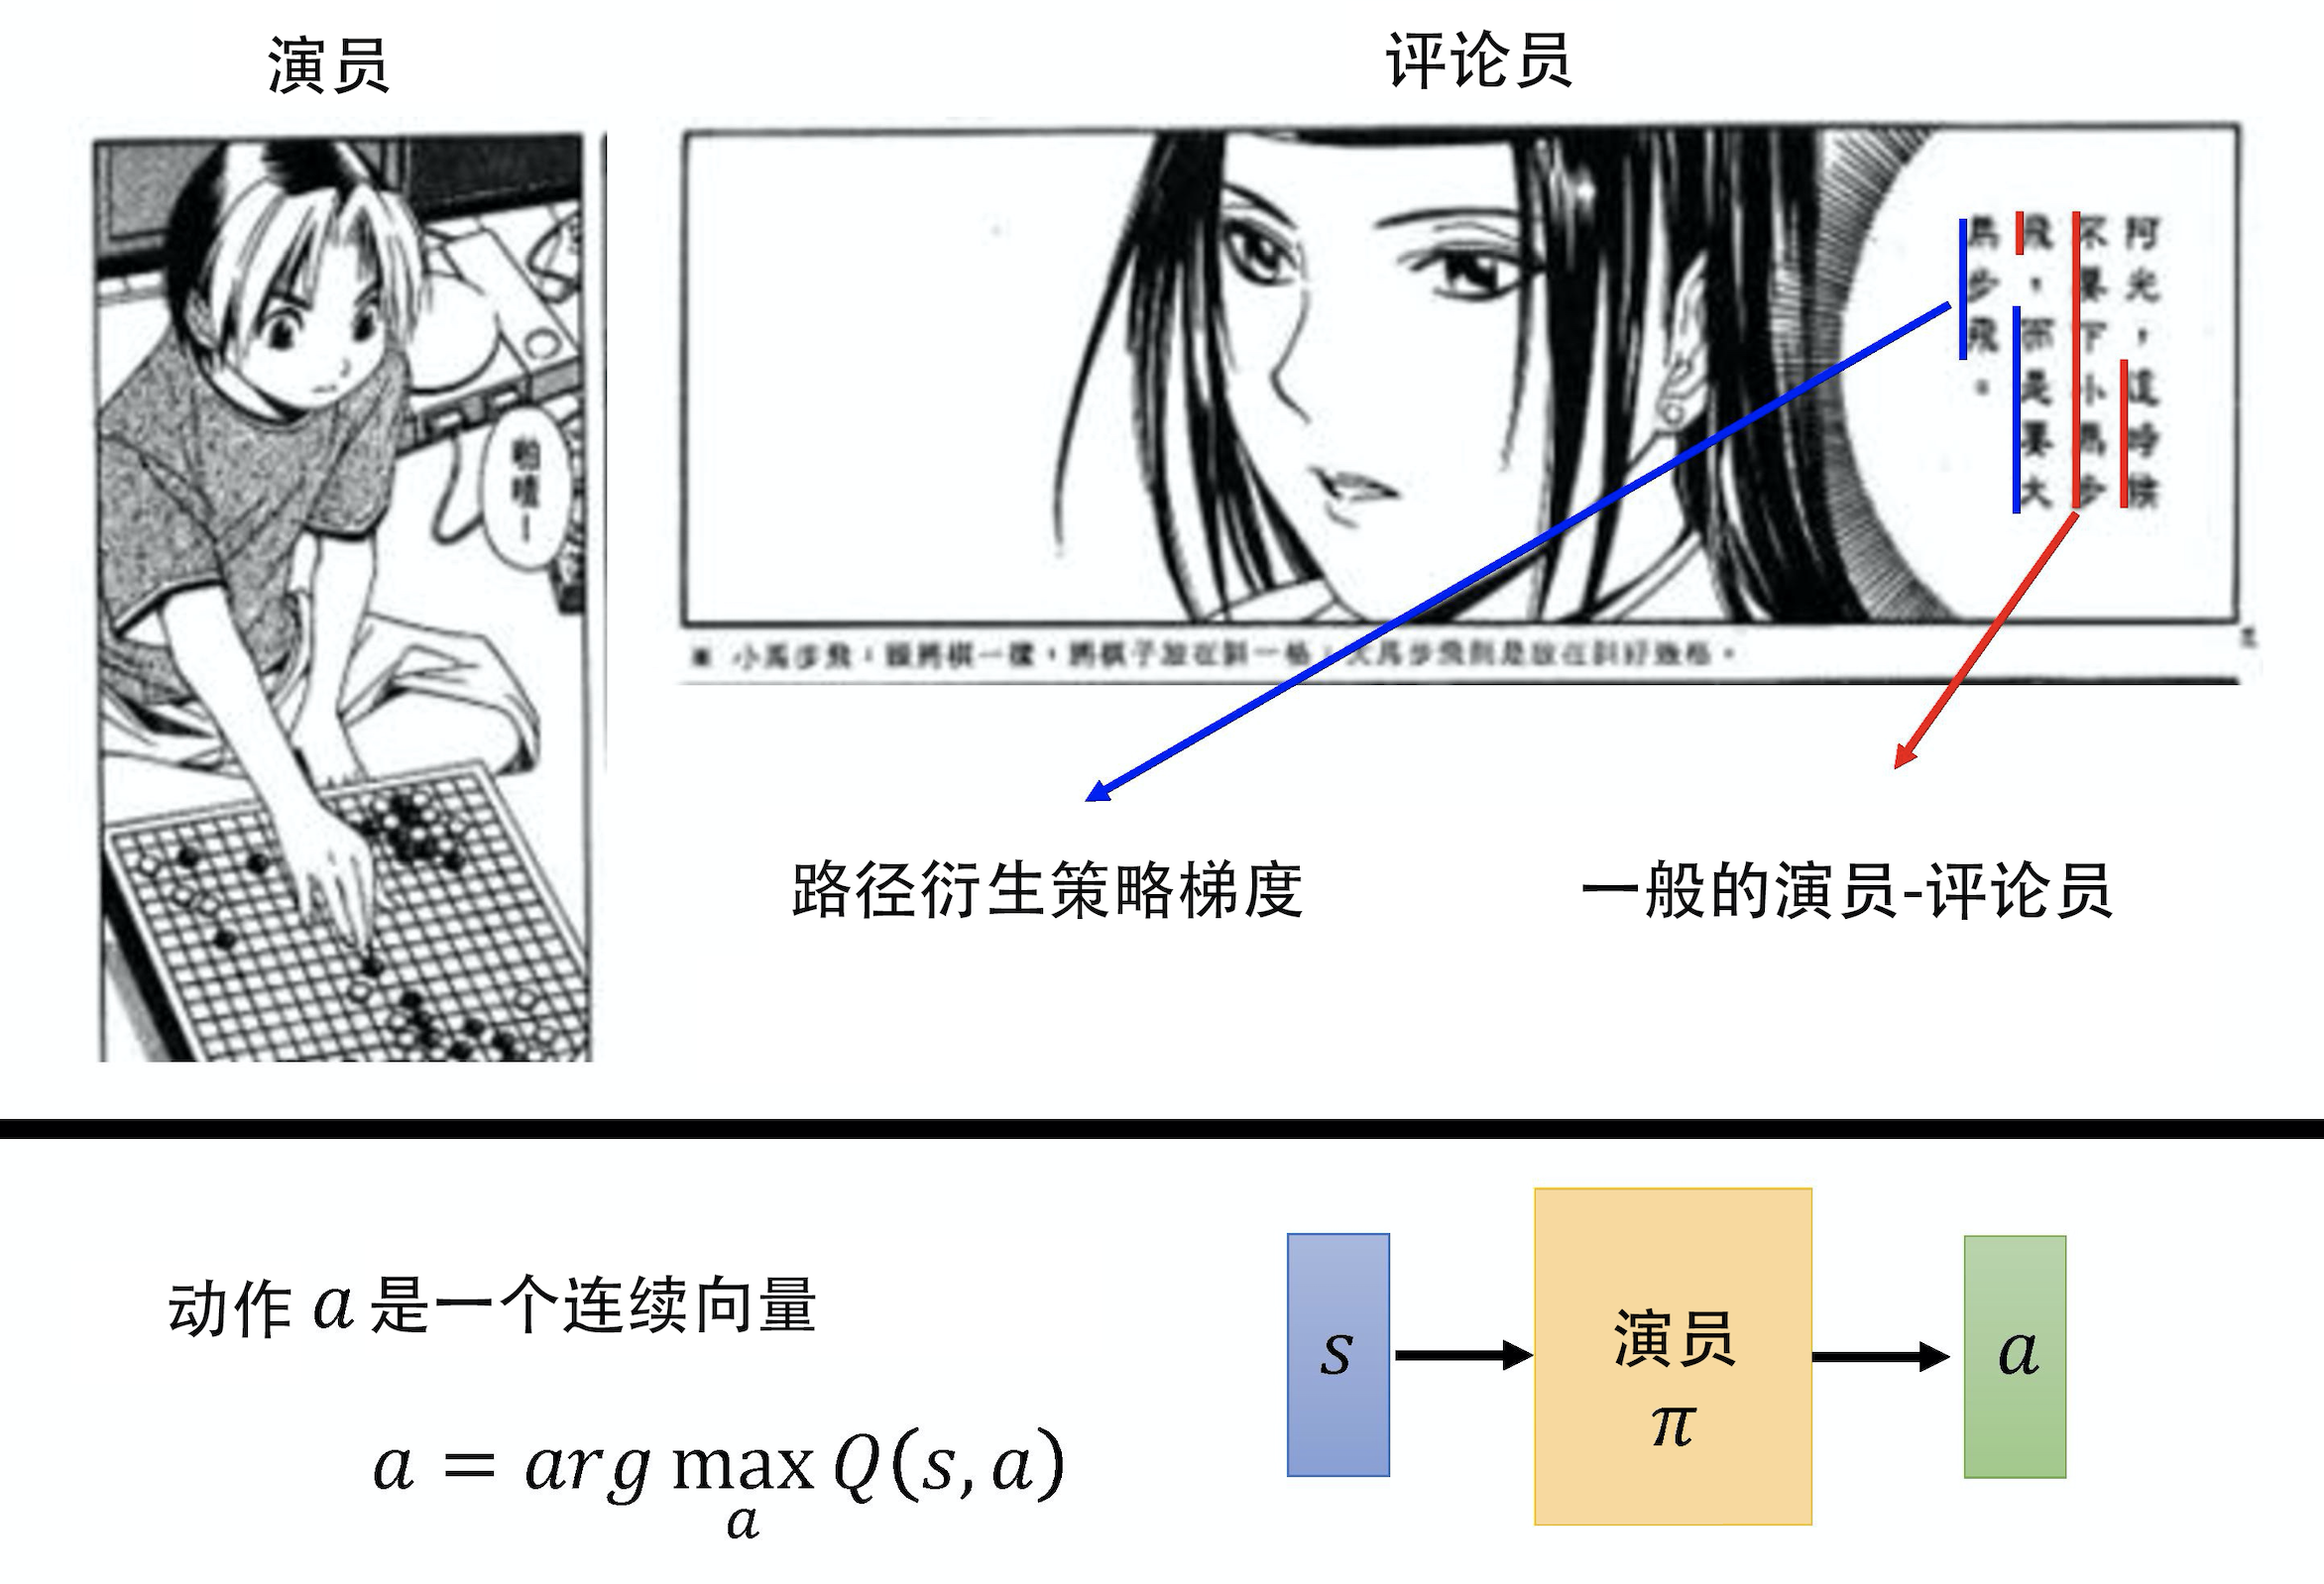
\includegraphics[width=0.7\linewidth]{res/ch9/9.9}
%   \caption{路径衍生策略梯度}
%   \label{fig:fig9.9}
% \end{figure}

从 深度Q网络 的观点来看,深度Q网络 的一个问题是在使用 深度Q网络 时,考虑连续向量会比较麻烦,没有通用的解决方法(general solution),那我们应该怎么解这个优化问题呢?
我们用一个演员来解决这个优化的问题。本来在深度Q网络 里面,如果是一个连续的动作,我们要解决这个优化问题。但是现在这个优化问题由演员来解决,假设演员就是一个解决者(solver),这个解决者的工作就是对于给定的状态 $s$,解出来哪一个动作可以得到最大的 Q 值,这是从另外一个观点来看路径衍生策略梯度。
在 生成对抗网络 中也有类似的说法。我们学习一个判别器(discriminator)并用于评估时,是非常困难的,因为我们要解决的 arg max 的问题非常的困难,所以用生成器(generator)来生成。
所以概念是一样的,Q 就是那个判别器。根据这个判别器决定动作非常困难,怎么办?另外学习一个网络来解决这个优化问题,这个网络就是演员。
所以两个不同的观点是同一件事。从两个不同的观点来看,
一个观点是:我们可以对原来的深度Q网络 加以改进,学习一个演员来决定动作以解决 arg max 不好解的问题。
另外一个观点是:原来的演员-评论员算法的问题是评论员并没有给演员足够的信息,评论员只告诉演员好或不好的,没有告诉演员什么样是好,现在有新的方法可以直接告诉演员什么样的是好的。
路径衍生策略梯度算法如\figref{fig:fig9.10} 所示,假设我们学习了一个Q函数,Q函数的输入是 $s$ 与 $a$,输出是 $Q_{\pi}(s,a)$。接下来,我们要学习一个演员,这个演员的工作就是解决 arg max 的问题,即输入一个状态 $s$,希望可以输出一个动作 $a$。$a$ 被代入Q函数以后,它可以让 $Q_{\pi}(s,a)$ 尽可能大,即
\begin{equation}
  \label{eq:}
  \pi^{\prime}(s)=\underset{a}{\arg \max} Q_{\pi}(s, a)
\end{equation}

实际上在训练的时候,我们就是把 Q 与演员连接起来变成一个比较大的网络。Q 是一个网络,接收输入 $s$ 与 $a$,输出一个值。演员在训练的时候,它要做的事就是接收输入 $s$,输出 $a$。把 $a$ 代入 Q 中,希望输出的值越大越好。我们会固定住 Q 的参数,只调整演员的参数,用梯度上升的方法最大化 Q 的输出,这就是一个 生成对抗网络,即有条件的生成对抗网络(conditional GAN)。Q 就是判别器,但在强化学习里就是评论员,演员在 生成对抗网络 里面就是生成器。

\begin{figure}[hbt]
  \centering
  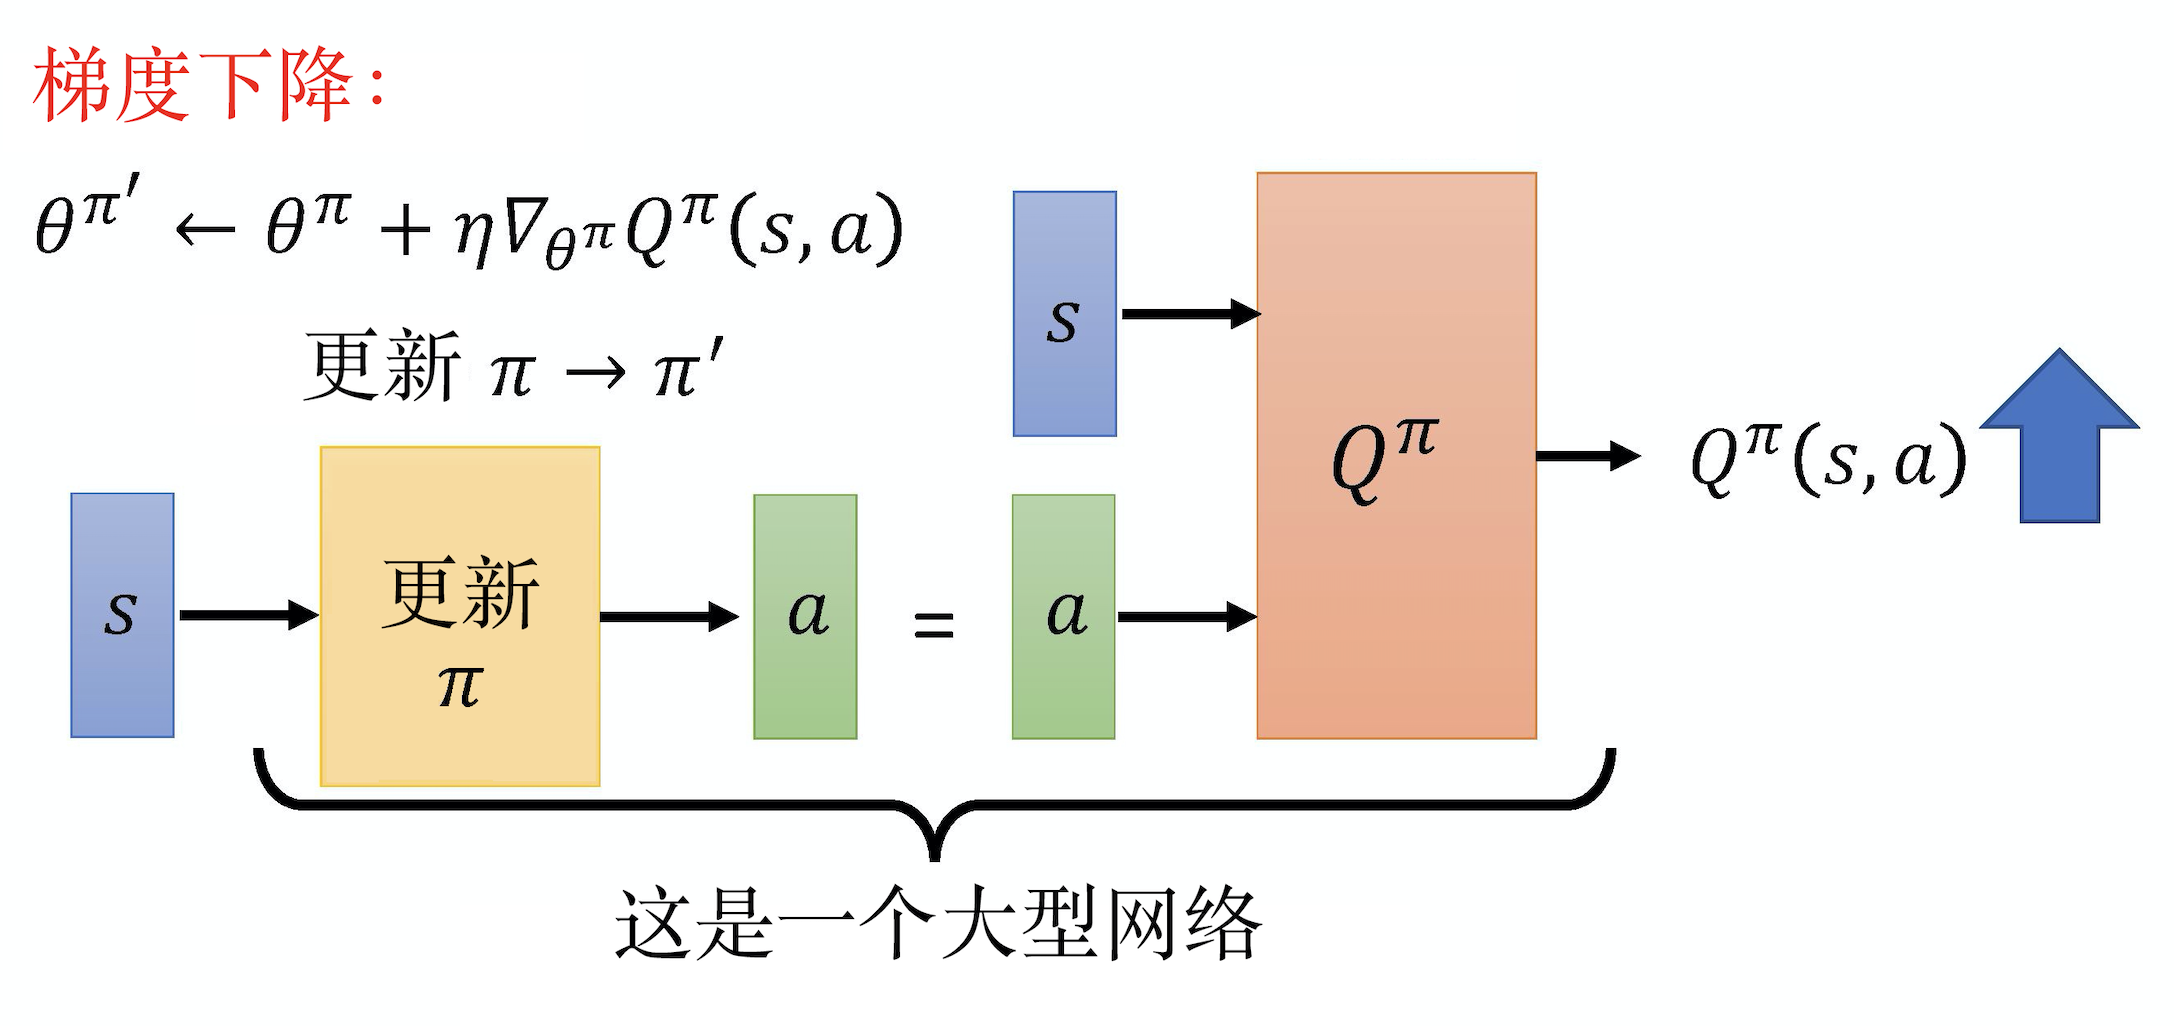
\includegraphics[width=0.5\linewidth]{res/ch9/9.10}
  \caption{路径衍生策略梯度}
  \label{fig:fig9.10}
\end{figure}


我们来看一下路径衍生策略梯度算法。如\figref{fig:fig9.11} 所示,一开始会有一个策略 $\pi$,它与环境交互并估计 Q 值。估计完 Q 值以后,我们就把 Q 值固定,只去学习一个演员。假设这个 Q 值估得很准,它知道在某一个状态采取什么样的动作会得到很大的Q值。接下来就学习这个演员,演员在给定 $s$ 的时候,采取了 $a$,可以让最后Q函数算出来的值越大越好。我们用准则(criteria)去更新策略 $\pi$,用新的 $\pi$ 与环境交互,再估计 Q值,得到新的 $\pi$ 去最大化 Q值的输出。深度Q网络 里面的技巧,在这里也几乎都用得上,比如经验回放、探索等技巧。

\begin{figure}[htb]
  \centering
  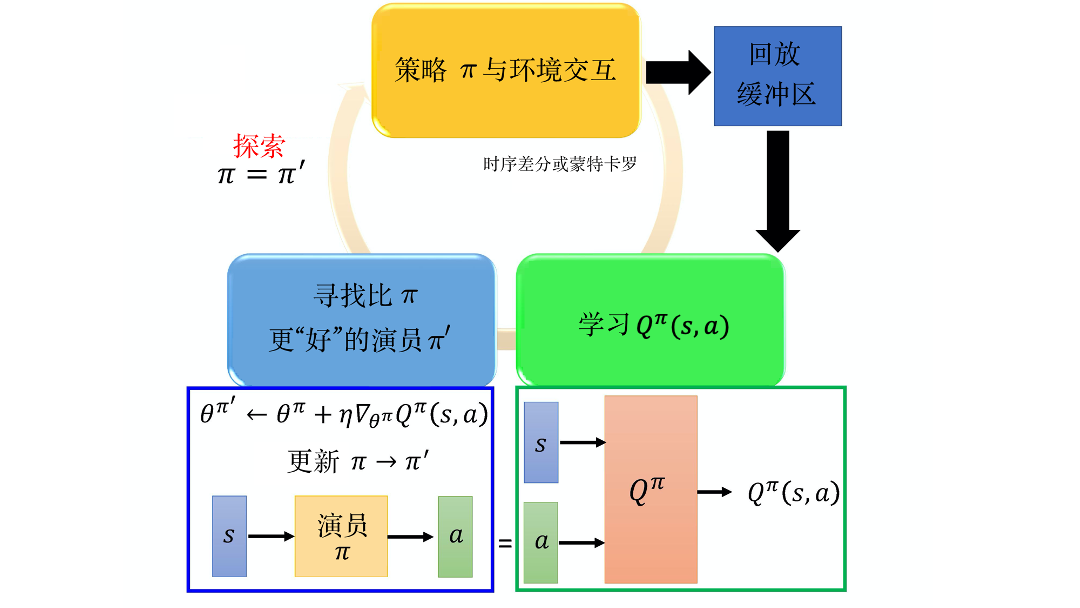
\includegraphics[width=0.5\linewidth]{res/ch9/9.11}
  \caption{路径衍生策略梯度算法}
  \label{fig:fig9.11}
\end{figure}

\figref{fig:fig9.12} 所示为原来深度Q网络 的算法。我们有一个Q函数 $Q$ 和另外一个目标Q函数 $\hat{Q}$。每一次训练,在每一个回合的每一个时间点,我们会看到一个状态 $s_t$,会采取某一个动作 $a_{t}$。至于采取哪一个动作是由Q函数所决定的。
如果是离散动作,我们看哪一个动作 $a$ 可以让 Q 值最大,就采取哪一个动作。当然,我们需要加一些探索,这样表现才会好。
我们会得到奖励 $r_t$,进入新的状态 $s_{t+1}$,然后把 $(s_t$,$a_{t}$,$r_t$,$s_{t+1})$ 放到回放缓冲区里。接下来,我们会从回放缓冲区中采样一个批量的数据,在这个批量数据里面,可能某一笔数据是 $(s_i, a_i, r_i, s_{i+1})$。接下来我们会算一个目标 $y$ ,$y=r_{i}+\max _{a} \hat{Q}\left(s_{i+1}, a\right)$。怎么学习 Q 呢?我们希望 $Q(s_i,a_i)$ 与 $y$ 越接近越好,这是一个回归问题,最后每 $C$ 步,要用 $Q$ 替代 $\hat{Q}$ 。

\begin{figure}[htb]
  \centering
  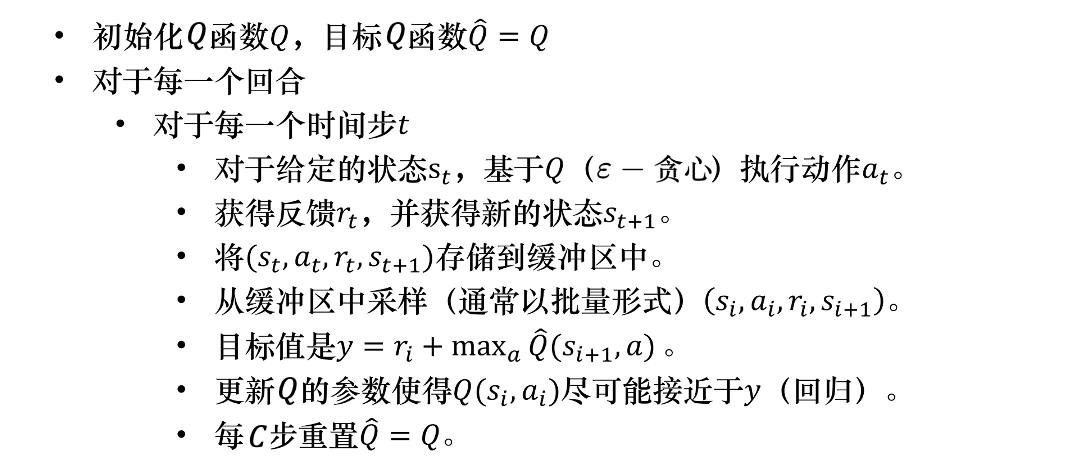
\includegraphics[width=0.5\linewidth]{res/ch9/9.12}
  \caption{深度Q网络算法}
  \label{fig:fig9.12}
\end{figure}

 接下来我们把深度Q网络 改成路径衍生策略梯度,需要做4个改变,如\figref{fig:fig9.13}所示。

(1)第一个改变是,我们要把 $Q$ 换成 $\theta$,本来是用 $Q$ 来决定在状态 $s_t$ 执行一个动作 $a_{t}$, 现在直接用 $\theta$ 来执行动作。
我们直接学习了一个演员。这个演员的输入 $s_t$ 会告诉我们应该采取哪一个 $a_{t}$。所以本来输入 $s_t$,采取哪一个 $a_t$是 Q 决定的,而在路径衍生策略梯度里面,我们会直接用 $\theta$ 来决定。

(2)第二个改变是,本来我们要计算在 $s_{i+1}$,根据策略采取某一个动作 $a$ 会得到的 Q 值,我们会采取让 $\hat{Q}$ 最大的那个动作 $a$。现在因为我们直接把 $s_{i+1}$ 代入$\theta$ ,就会知道给定 $s_{i+1}$ ,哪个动作会给我们最大的 Q值,就采取哪个动作。
在Q函数里面,有两个Q网络:真正的 Q网络和目标 Q 网络。实际上我们在实现路径衍生策略梯度算法的时候,也有两个演员:真正要学习的演员$\theta$和目标演员$\hat{\theta}$。这个原理就与为什么要有目标 Q 网络一样,我们在算目标值的时候,并不希望它一直的变动,所以我们会有一个目标演员和一个目标Q函数,它们平常的参数就是固定住的,这样可以让目标的值不会一直地变化。
% 所以本来到底是要用哪一个动作 $a$,我们会看说哪一个动作 $a$ 可以让 $\hat{Q}$  最大。但现在因为哪一个动作 $a$ 可以让 $\hat{Q}$ 最大这件事情已经用策略取代掉了,所以我们要知道哪一个动作 $a$ 可以让 $\hat{Q}$ 最大,就直接把那个状态代入 $\hat{\pi}$ 里面,看它得到哪一个 $a$,那个 $a$ 就是会让 $\hat{Q}(s,a)$ 的值最大的那个 $a$ 。
% 其实与原来的 深度Q网络 也是没什么不同,
总结一下,第二个改变是我们用策略取代原来要解 arg max 的地方。

(3)第三个改变是,之前只要学习 Q函数,现在我们多学习了一个 $\theta$,学习 $\theta$ 的目的是最大化Q函数,希望得到的演员可以让Q函数的输出尽可能大,这与学习 生成对抗网络 里面的生成器的概念是类似的。

(4)第四个改变是,我们不仅要取代目标的 Q 网络,还要取代目标策略。

\begin{figure}[hbt]
  \centering
  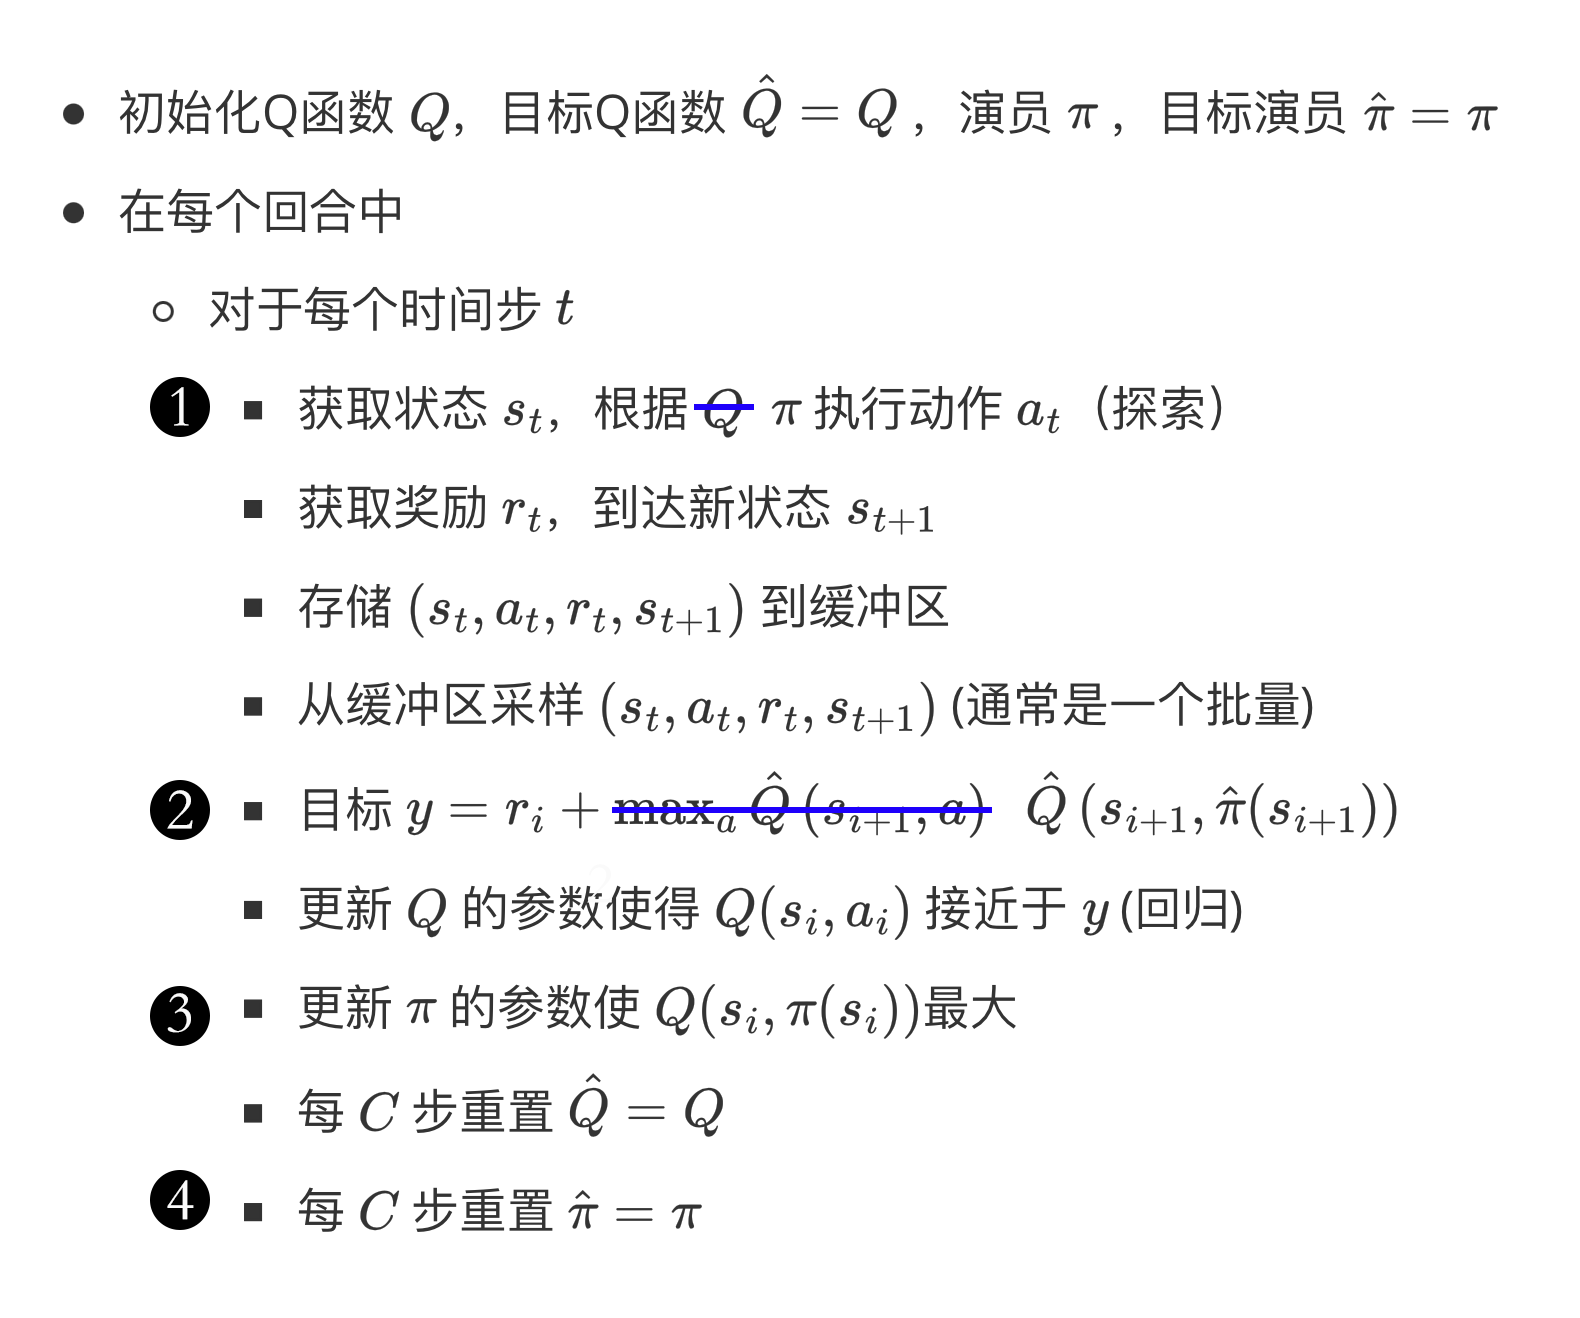
\includegraphics[width=0.5\linewidth]{res/ch9/9.13}
  \caption{从深度Q网络到路径衍生策略梯度}
  \label{fig:fig9.13}
\end{figure}

\subsection{与生成对抗网络的联系} 

如\tabref{tab:GAN_AC} 所示,GAN 与演员-评论员的方法是非常类似的。如果大家感兴趣,可以参考一篇论文:“Connecting Generative Adversarial Network and Actor-Critic Methods”。

生成对抗网络 与演员-评论员都挺难训练,所以在文献上就有各式各样的方法,告诉我们怎么样可以训练 生成对抗网络。
知道 生成对抗网络 与演员-评论员非常相似后,我们就可以知道怎样训练演员-评论员。但是因为做 生成对抗网络 与演员-评论员的人是两群人,所以这篇论文里面就列出说在 生成对抗网络 上面有哪些技术是有人做过的,在演员-评论员上面,有哪些技术是有人做过的。也许训练 生成对抗网络 的技术,我们可以试着应用在演员-评论员上,在演员-评论员上用过的技术,也可以试着应用在 生成对抗网络 上。

\begin{table}[hbt]
  \caption{与生成对抗网络的联系}
  \label{tab:GAN_AC}
  \centering
  \begin{tabular}{ccc}
  \toprule
  方法    & 生成对抗网络 & 演员-评论员 \\ \hline
  冻结学习  & 有      &  有    \\ 
  标签平滑  & 有     & 无      \\
  历史平均  &  有    & 无     \\ 
  小批量判别 &  有    & 无      \\ 
  批量归一化 &  有   &  有    \\ 
  目标网络  & 不适用    & 有      \\ 
  经验回放  & 无      & 有     \\ 
  熵正则化  & 无      & 有    \\ 
  兼容性   & 无      &  有   \\ 
  \bottomrule
  \end{tabular}
  \end{table}

% \begin{figure}[hbt]
%   \centering
%   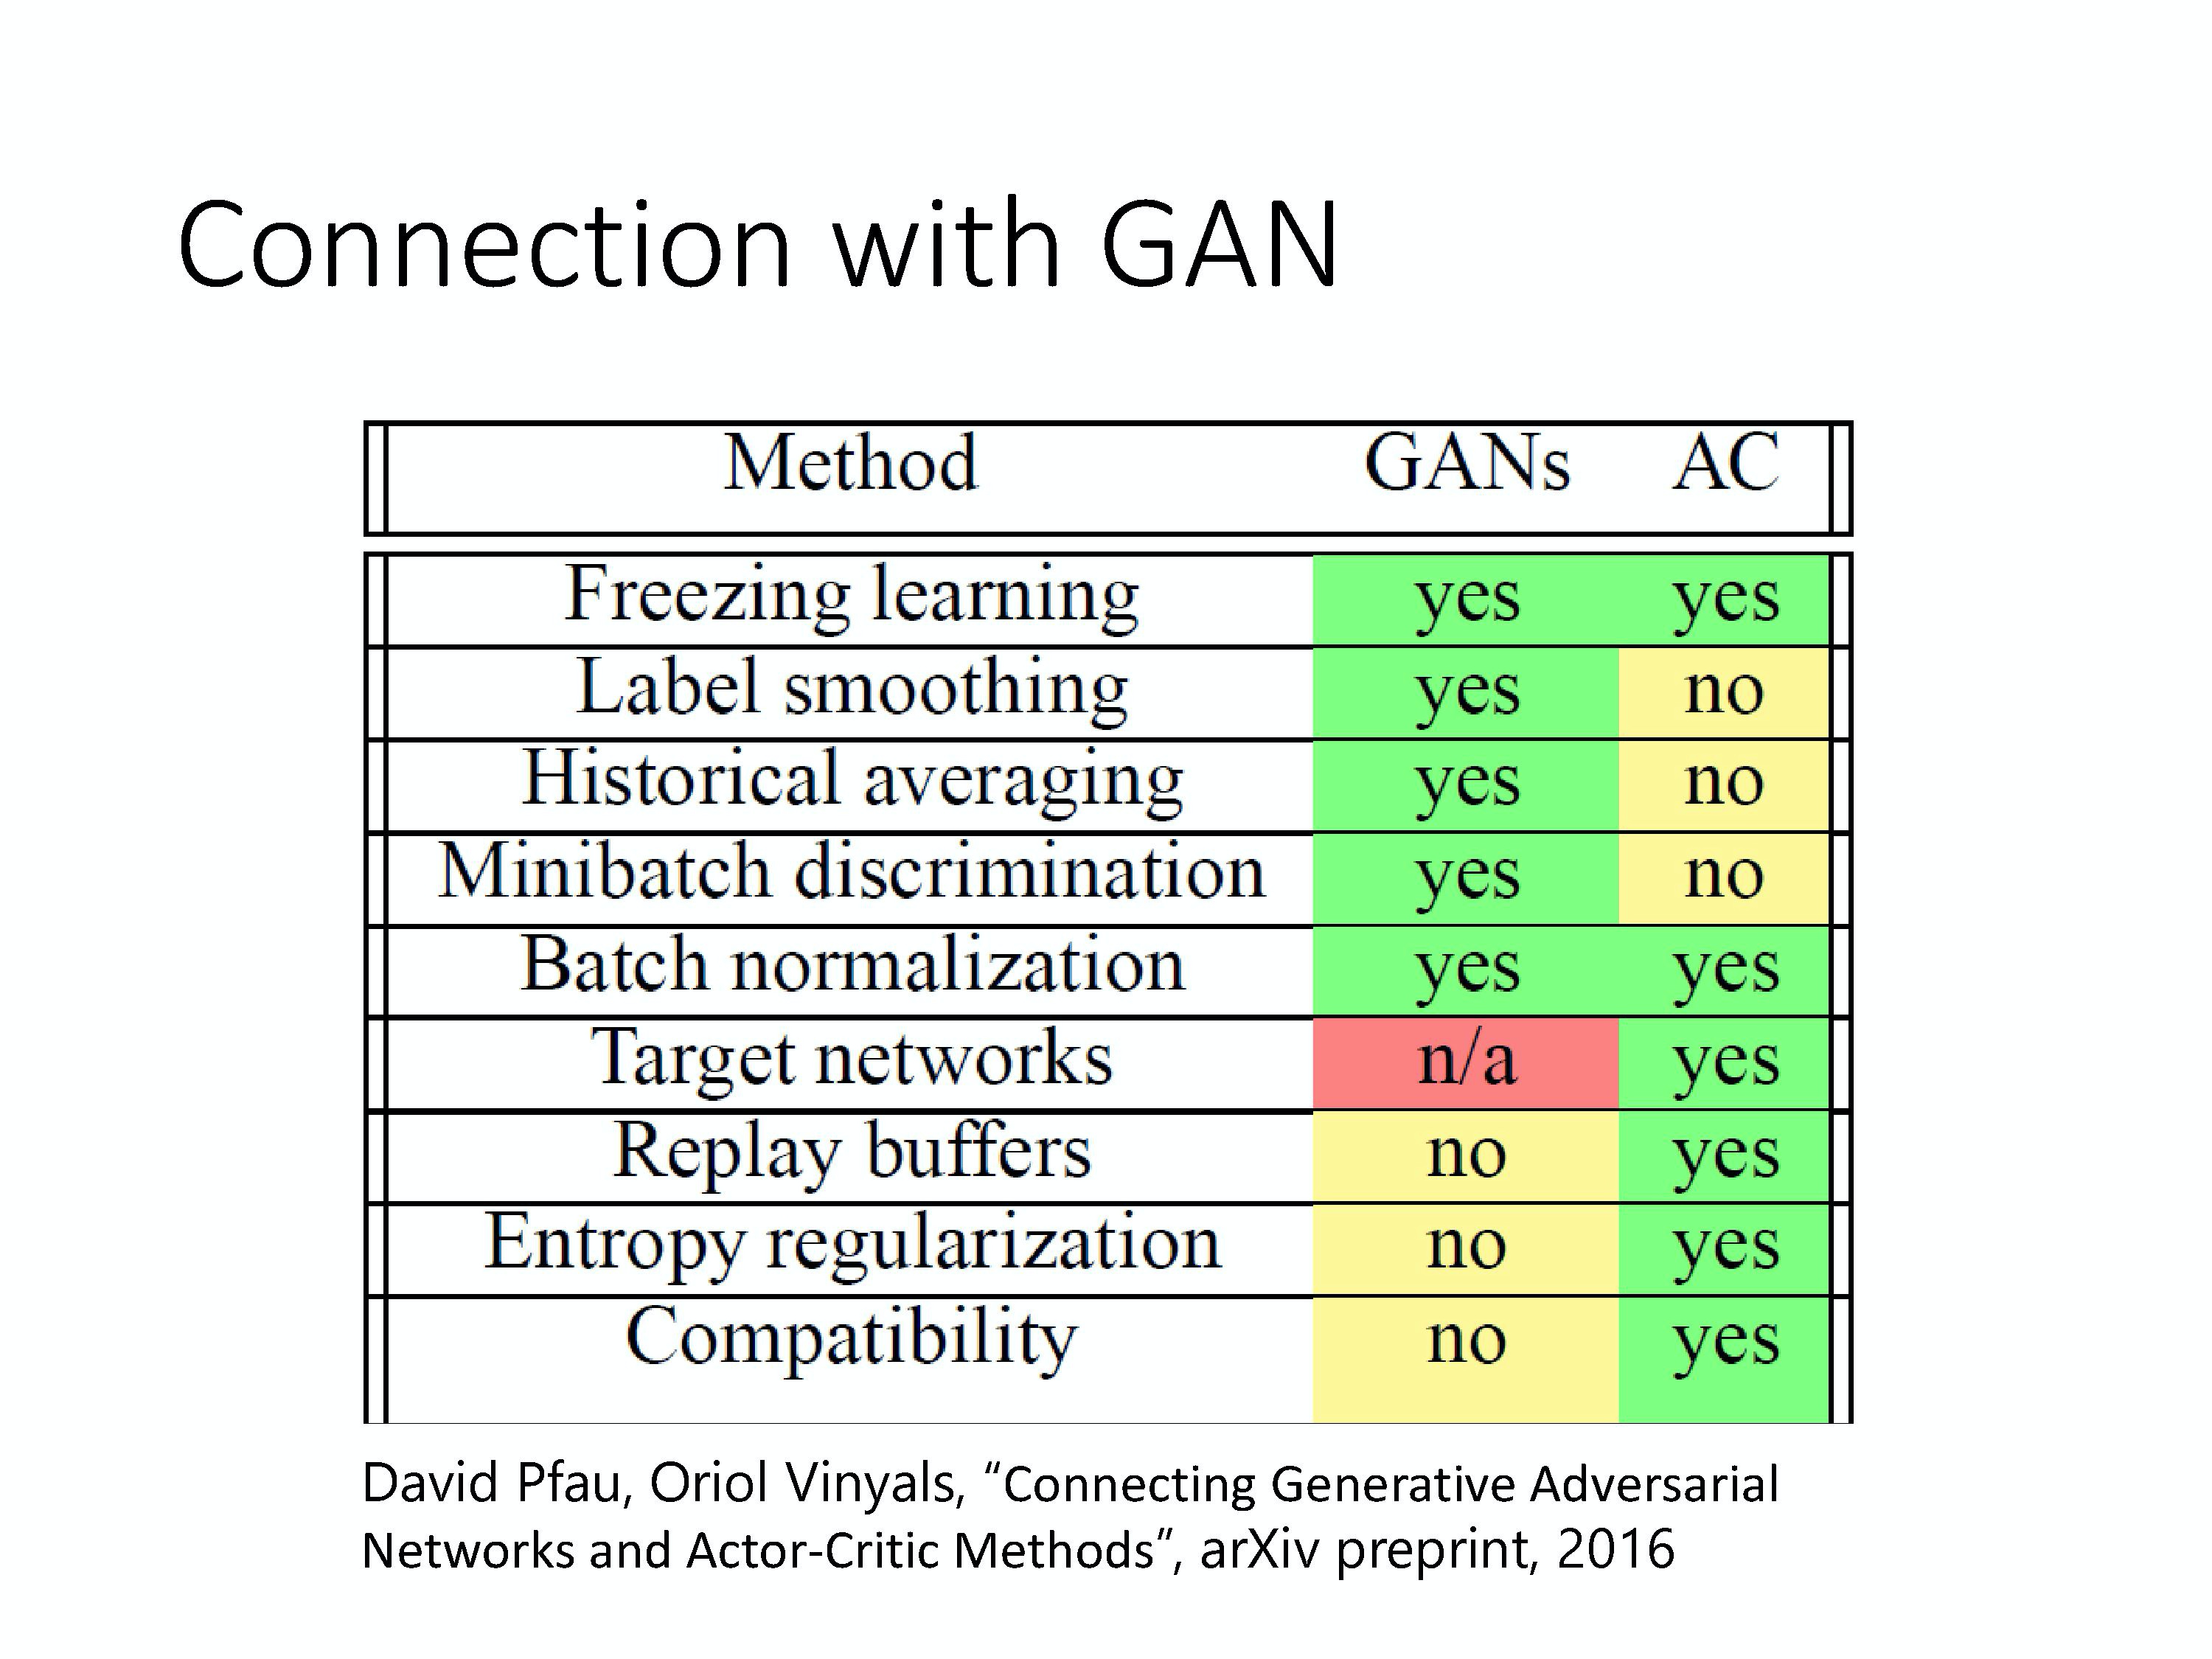
\includegraphics[width=0.7\linewidth]{res/ch9/9.14}
%   \caption{与生成对抗网络的联系}
%   \label{fig:fig9.14}
% \end{figure}

\subsection{关键词}

优势演员-评论员(advantage actor-critic,A2C)算法:一种改进的演员-评论员(actor-critic)算法。

异步优势演员-评论员(asynchronous advantage actor-critic,A3C)算法:一种改进的演员-评论员算法,通过异步的操作,实现强化学习模型训练的加速。

路径衍生策略梯度(pathwise derivative policy gradient):一种使用Q学习来求解连续动作的算法,也是一种演员-评论员算法。其会对演员提供价值最大的动作,而不仅仅是提供某一个动作的好坏程度。


\subsection{习题}

\kw{9-1} 完整的优势演员-评论员算法的工作流程是怎样的?

\kw{9-2} 在实现演员-评论员算法的时候有哪些技巧?

\kw{9-3} 异步优势演员-评论员算法在训练时有很多的进程进行异步的工作,最后再将他们所获得的“结果”集合到一起。那么其具体是如何运作的呢?

\kw{9-4} 对比经典的Q学习算法,路径衍生策略梯度有哪些改进之处?

 
\subsection{面试题}

\kw{9-1} 友善的面试官:请简述一下异步优势演员-评论员算法(A3C),另外A3C是同策略还是异策略的模型呀?

\kw{9-2} 友善的面试官:请问演员-评论员算法有何优点呢?

\kw{9-3} 友善的面试官:请问异步优势演员-评论员算法具体是如何异步更新的?

\kw{9-4} 友善的面试官:演员-评论员算法中,演员和评论员两者的区别是什么?

\kw{9-5} 友善的面试官:演员-评论员算法框架中的评论员起了什么作用?

\kw{9-6} 友善的面试官:简述异步优势演员-评论员算法的优势函数。
  


% \subsection*{参考文献} 
% \begin{itemize}
%     \item \href{https://nndl.github.io/}{神经网络与深度学习}
% \end{itemize}


